%!TEX root = ../TemplateMasterThesis.tex

\chapter{Chapter Two} % (fold)
\label{cha:chapter_two}

\section{Section about figures} % (fold)
\label{sec:section_about_figures}

This is an example how you can include a figure

\begin{figure}[!ht]
	\centering
		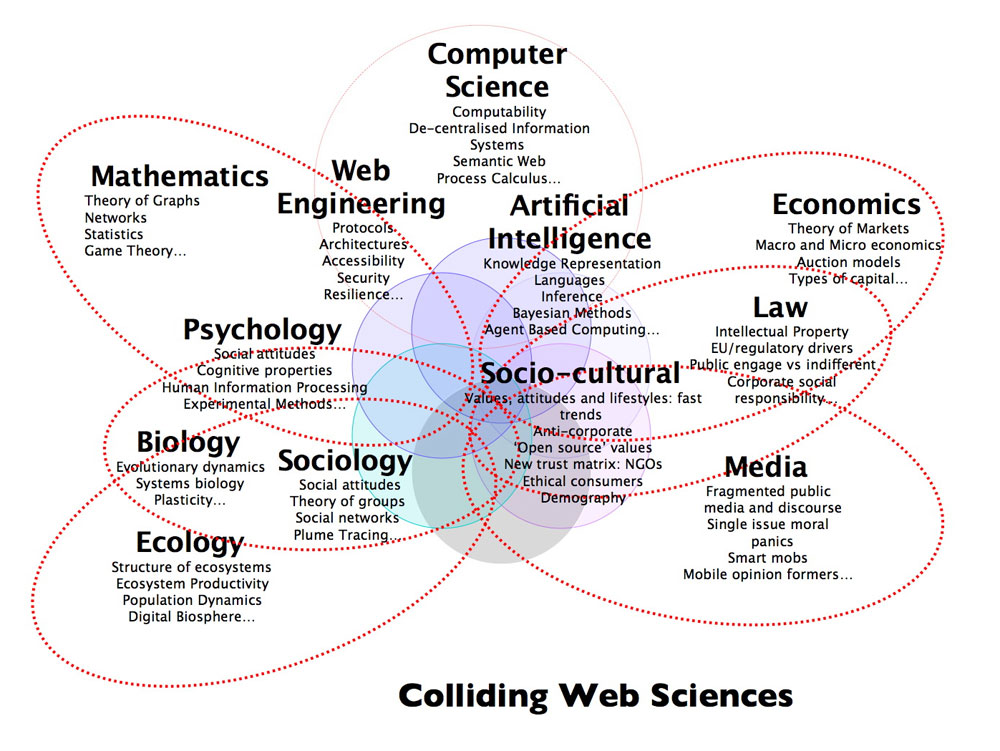
\includegraphics[height=3in]{images/webscience.jpg}
	\caption{Here you insert the caption of the figure \citep{Stanford09}}
	\label{fig:images_webscience}
\end{figure}

It is also important to indicate the source of the figure. In this case in the bibtex file a online resource is inserted and referred to here.

% section section_about_figures (end)


\section{Section about quotations} % (fold)
\label{sec:section_about_quotations}

In this section, an example for a literal quotation is given. 

\begin{quotation}
	\emph{``A persona is a rich picture of an imaginary person who represents your core user group.''}
	\citep{Dix04}
\end{quotation}

Alternative you can also write it like this:

\begin{quotation}
	\textit{\enquote{A persona is a rich picture of an imaginary person who represents your core user group.}} \citep{Dix04}
\end{quotation}

The compiled output remains the same. \\

Sometimes you might want to make use of the authors name within the text. Before, we used the command \texttt{citep\{\}}, which creates the brackets around author name and year. You can also use the \texttt{cite} command like this: \\

\cite{Dix04} defined the concept of persona as follows: 
\begin{quotation}
	\emph{``A persona is a rich picture of an imaginary person who represents your core user group.''}
	\citep{Dix04}
\end{quotation}

You may notice, that this increases the readability of the text. \\

According to APA format\footnote{ American Psychological Association (APA)} there are some rules, when and how to include page numbers, when referring to literature. 

\begin{quotation}
	\emph{``Include page numbers for any citations in the text of your paper that include direct quotations or refer to a specific part of the work you are referencing. Direct quotations must include a page number as part of the citation. The quoted material should be followed by a citation in parentheses that gives the author's name, the year in which the work was published, and the page number from which the quoted material appears.''}
	\citep{Hall}
\end{quotation}

Check out the example and recommendations of \cite{Hall} on \url{http://www.ehow.com/how_5689799_cite-numbers-apa-format.html}. In \LaTeX you can include the pages very easy. For example: \\

\citet[p. 86]{Baddeley:1974ts} stated: 

\begin{quotation}
	\emph{``We hope that our preliminary attempts to begin answering the question will convince the reader, not necessarily that our views are correct, but that the question was and is well worth asking''}
	\citep[p. 86]{Baddeley:1974ts}
\end{quotation}

Note that in the first reference, we used \texttt{citet[]\{\}} in order to have brackets just around year and page number; later we used \texttt{citep[]\{\}}.

% section section_about_quotations (end)


\section{Section about references within the document} % (fold)
\label{sec:section_about_references_within_the_document}

If you want to refer to you own chapters, figures, tables or the like, you can make use of the \texttt{ref\{\}} command, like we did in section~\ref{sec:section_in_which_the_tables_are_referred_to} on page \pageref{sec:section_in_which_the_tables_are_referred_to}. \\

Here we refer to figure~\ref{fig:images_webscience} on page \pageref{fig:images_webscience}. As you may notice, when you take a look at the \LaTeX{} Code, you don't have to check the page numbering, even if you re-structure your document. We use the \texttt{pageref\{\}} command for that.




% section section_about_references_within_the_document (end)


% chapter chapter_two (end)


